%%%%%%%%%%%%%%%%%%%%%%%%%%%%% Define Article %%%%%%%%%%%%%%%%%%%%%%%%%%%%%%%%%%
\documentclass[conference]{IEEEtran}
%%%%%%%%%%%%%%%%%%%%%%%%%%%%%%%%%%%%%%%%%%%%%%%%%%%%%%%%%%%%%%%%%%%%%%%%%%%%%%%

%%%%%%%%%%%%%%%%%%%%%%%%%%%%% Using Packages %%%%%%%%%%%%%%%%%%%%%%%%%%%%%%%%%%
\usepackage{geometry}
\usepackage{graphicx}
\usepackage{amssymb}
\usepackage{amsmath}
\usepackage{amsthm}
\usepackage{empheq}
\usepackage{mdframed}
\usepackage{booktabs}
\usepackage{lipsum}
\usepackage{graphicx}
\usepackage{psfrag}
\usepackage{pgfplots}
\usepackage{bm}
\usepackage[spanish]{babel}
\usepackage[utf8]{inputenc} % Codificación UTF,8
\usepackage{amsmath}        % Soporte para ecuaciones matemáticas
\usepackage{graphicx}       % Manejo de imágenes
\usepackage{hyperref}       % Hipervínculos
\usepackage{caption}        % Formato para figuras
\usepackage{multirow}
\usepackage{subcaption}
\usepackage{biblatex} % Add the bibliography file in the preamble (correct usage)
\usepackage{csquotes}
\usepackage{bookmark}
%%%%%%%%%%%%%%%%%%%%%%%%%%%%%%%%%%%%%%%%%%%%%%%%%%%%%%%%%%%%%%%%%%%%%%%%%%%%%%%
\usepackage{listings}
\usepackage{color}
% \usepackage{colors} % Removed because 'colors' package does not exist
% Other Settings

%%%%%%%%%%%%%%%%%%%%%%%%%% Page Setting %%%%%%%%%%%%%%%%%%%%%%%%%%%%%%%%%%%%%%%
\geometry{a4paper, margin=1in}

%%%%%%%%%%%%%%%%%%%%%%%%%% Define some useful colors %%%%%%%%%%%%%%%%%%%%%%%%%%
\definecolor{ocre}{RGB}{243,102,25}
\definecolor{mygray}{RGB}{243,243,244}
\definecolor{deepGreen}{RGB}{26,111,0}
\definecolor{shallowGreen}{RGB}{235,255,255}
\definecolor{deepBlue}{RGB}{61,124,222}
\definecolor{shallowBlue}{RGB}{235,249,255}
    
\definecolor{codegreen}{rgb}{0,0.6,0}
\definecolor{codegray}{rgb}{0.5,0.5,0.5}
\definecolor{codepurple}{rgb}{0.58,0,0.82}
\definecolor{codeblue}{rgb}{0,0,0.8}    
\definecolor{backcolour}{rgb}{0.98, 0.98, 0.98}
%%%%%%%%%%%%%%%%%%%%%%%%%%%%%%%%%%%%%%%%%%%%%%%%%%%%%%%%%%%%%%%%%%%%%%%%%%%%%%%

%%%%%%%%%%%%%%%%%%%%%%%%%% Define an orangebox command %%%%%%%%%%%%%%%%%%%%%%%%
\newcommand\orangebox[1]{\fcolorbox{ocre}{mygray}{\hspace{1em}#1\hspace{1em}}}
%%%%%%%%%%%%%%%%%%%%%%%%%%%%%%%%%%%%%%%%%%%%%%%%%%%%%%%%%%%%%%%%%%%%%%%%%%%%%%%

%%%%%%%%%%%%%%%%%%%%%%%%%%%% English Environments %%%%%%%%%%%%%%%%%%%%%%%%%%%%%
\newtheoremstyle{mytheoremstyle}{3pt}{3pt}{\normalfont}{0cm}{\rmfamily\bfseries}{}{1em}{{\color{black}\thmname{#1}~\thmnumber{#2}}\thmnote{\,,,\,#3}}
\newtheoremstyle{myproblemstyle}{3pt}{3pt}{\normalfont}{0cm}{\rmfamily\bfseries}{}{1em}{{\color{black}\thmname{#1}~\thmnumber{#2}}\thmnote{\,,,\,#3}}
\theoremstyle{mytheoremstyle}
\newmdtheoremenv[linewidth=1pt,backgroundcolor=shallowGreen,linecolor=deepGreen,leftmargin=0pt,innerleftmargin=20pt,innerrightmargin=20pt,]{theorem}{Theorem}[section]
\theoremstyle{mytheoremstyle}
\newmdtheoremenv[linewidth=1pt,backgroundcolor=shallowBlue,linecolor=deepBlue,leftmargin=0pt,innerleftmargin=20pt,innerrightmargin=20pt,]{definition}{Definition}[section]
\theoremstyle{myproblemstyle}
\newmdtheoremenv[linecolor=black,leftmargin=0pt,innerleftmargin=10pt,innerrightmargin=10pt,]{problem}{Problem}[section]
%%%%%%%%%%%%%%%%%%%%%%%%%%%%%%%%%%%%%%%%%%%%%%%%%%%%%%%%%%%%%%%%%%%%%%%%%%%%%%%

%%%%%%%%%%%%%%%%%%%%%%%%%%%%%%% Plotting Settings %%%%%%%%%%%%%%%%%%%%%%%%%%%%
\usepgfplotslibrary{colorbrewer}
\pgfplotsset{width=8cm,compat=1.9}
%%%%%%%%%%%%%%%%%%%%%%%%%%%%%%%%%%%%%%%%%%%%%%%%%%%%%%%%%%%%%%%%%%%%%%%%%%%%%%%

%%%%%%%%%%%%%%%%%%%%%%%%%%%%%%% Title & Author %%%%%%%%%%%%%%%%%%%%%%%%%%%%%%%%
\author{\IEEEauthorblockN{Daniel Fernando Aranda Contreras}
\IEEEauthorblockA{Escuela E3T, Universidad Industrial de Santander\\
Correo electrónico: \{daniel2221648 \}@correo.uis.edu.co}}

%%%%%%%%%%%%%%%%%%%%%%%%%%%%%%%%%%%%%%%%%%%%%%%%%%%%%%%%%%%%%%%%%%%%%%%%%%%%%%%
    % Definición de colores para el estilo de MATLAB
    \lstdefinestyle{MATLABStyle}{
        backgroundcolor=\color{backcolour},   
        commentstyle=\color{codegreen},
        keywordstyle=\color{codeblue},
        numberstyle=\tiny\color{codegray},
        stringstyle=\color{codepurple},
        basicstyle=\ttfamily\footnotesize,
        breakatwhitespace=false,         
        breaklines=true,                 
        captionpos=b,                    
        keepspaces=true,                 
        numbers=left,                    
        numbersep=5pt,                  
        showspaces=false,                
        showstringspaces=false,
        showtabs=false,                  
        tabsize=2,
        linewidth=0.48\textwidth,
            %frame=single,
    }
    \lstset{language=Matlab, style=MATLABStyle}
%%%%%%%%%%%%%%%%%%%%%%%%%%%%%%%%%%%%%%%%%%%%%%%%%%%%%%%%%%%%%%%%%%%%%%%%%%%%%%%
    \begin{document}


        % Título
        \title{\uppercase{Diseño implementacioón y desarrollo de una intefaz para motores de inducción}}
        \maketitle
        % Resumen
        % Palabras clave        
        \begin{IEEEkeywords}
            Motor de Inducción,
            Interfaz Gráfica de Usuario (GUI),
            MATLAB App Designer,
            Cálculo de Parámetros,
            Máquinas Eléctricas,
            Modelado de Motores,
            Rendimiento Energético,
            Deslizamiento,
            Potencia (Eléctrica),
            Par Motor.
        \end{IEEEkeywords}



        \begin{abstract}
        This report details the design, implementation, and development of a graphical user interface (GUI), created using MATLAB App Designer, for the simulation and calculation of induction motor parameters. The interface facilitates the input of crucial data such as iron and stray losses, stator and rotor resistances and reactances, source voltage, frequency, number of poles, and slip.     
        \end{abstract}
        %\section{Objetivos} 
\begin{itemize}
    \item Realizar las pruebas de vacío y de cortocircuito en un transformador monofásico configurado como autotransformador para analizar su comportamiento eléctrico.
    \item Determinar experimentalmente el rendimiento y la regulación del autotransformador bajo diferentes tipos de carga: resistiva, inductiva y capacitiva.
\end{itemize}

\section{Equiops y materiales}
\begin{itemize}
    \item Transformador monofásico.
    \item Voltímetro CA.
    \item Amperímetro CA.
    \item Vatímetro monofásico CA.
    \item Transformador de corriente (CT).
    \item Cargas: resistivas (R), inductivas (L) y capacitivas (C).
\end{itemize}

\section{Introducción}
\text{Los autotransformadores son dispositivos eléctricos que facilitan la modificación de los niveles de tensión dentro de un rango específico de manera eficiente. A diferencia de los transformadores tradicionales, en los autotransformadores los devanados primario y secundario no están completamente aislados, ya que comparten una parte del mismo arrollamiento. Esto resulta en una reducción del material conductor utilizado y en una mejora de la eficiencia del sistema. En este laboratorio, se realizará un estudio de un transformador monofásico funcionando como autotransformador, a través de pruebas experimentales que permitirán evaluar su rendimiento y regulación en diversas condiciones de carga.}

\section{Conclusión}
\text{A lo largo del laboratorio, se estudió el comportamiento de un transformador monofásico operando como autotransformador, evaluando su rendimiento y regulación bajo diferentes condiciones de carga, las cuales tienen una gran influencia en su rendimiento depediendo el tipo de carga, si es una carga RC conectada en paralelo tiende a aunmentar su tension de salida en comparacion con una carga netamente resistiva, mientras que con una carga inductiva conectada en serie su nivel de tension de salida disminuye, pero si conectamos una carga RLC está tiene un comportamiento de compensacion, si las cargas inductivas (L) y capacitivas (C) tienen valores similares.}

        \section{Introducción}
La interfaz busca implementar un método numérico mediante App Designer de MATLAB que ayude a identificar aspectos de funcionamiento y emule el comportamiento de un motor de inducción en estado estacionario. Para unas entradas y salidas ya definidas. El alcance del proyecto no busca ser un método más preciso al empleado en la literatura y diversos libros de máquinas eléctricas; al contrario, toma como apoyo dichas ecuaciones ya definidas.

\section{Resumen}
Las máquinas de inducción, particularmente los motores trifásicos, son fundamentales en la industria debido a su robustez, eficiencia y bajo mantenimiento. Para comprender su comportamiento y características operativas, es esencial realizar ensayos experimentales que permitan analizar su rendimiento en distintas condiciones. Entre las pruebas más comunes se encuentran la prueba de vacío y la prueba de rotor bloqueado, las cuales proporcionan información clave para la obtención de los parámetros del equivalente eléctrico del motor. Para la creación del codigo ya se parte de un equivalente de dichas pruebas realizadas y del modelo del circiuto se tienen las entradas y a partir de estas entradas hallar las salidas se tomó un modelo de motor ya definido en la literatura —con su significado físico—. Se concatenaron las ecuaciones del modelo en función de las entradas y salidas definidas.


        \section{Principio de funcionamiento entorno matlab y aspectos relacionados con las ecuaciones} 
\subsection{modelo del circuito empleado}

\begin{figure}[ht!]
    \centering
    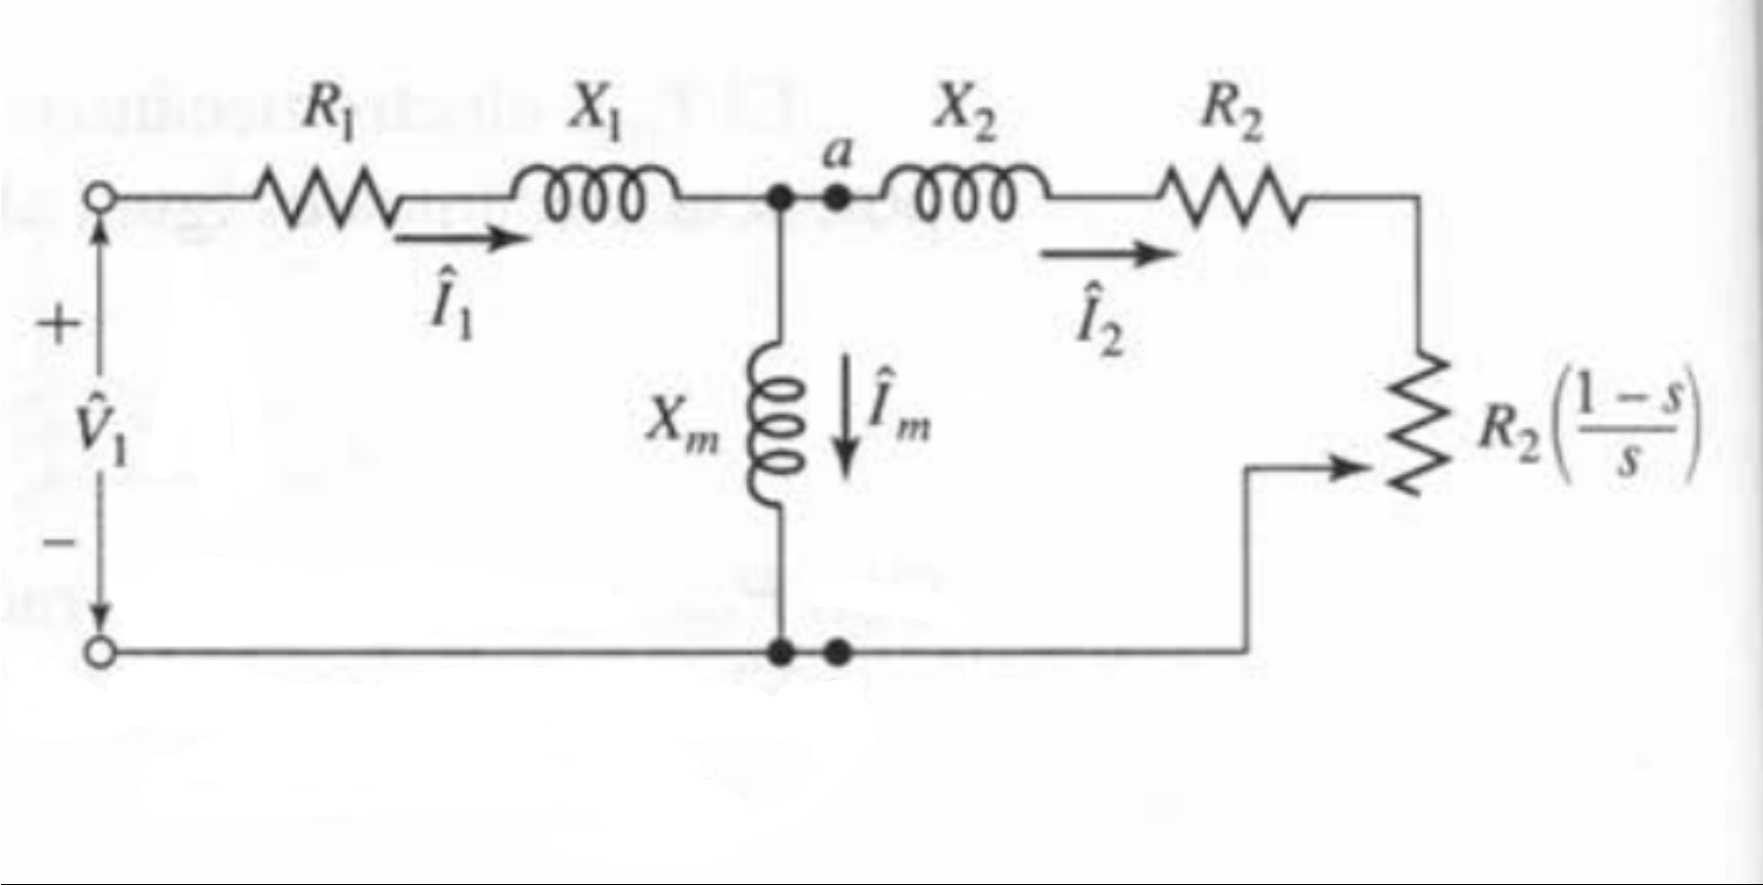
\includegraphics[width=0.48\textwidth]{imginterfaz/circuito equivalente.png}
    \caption{Modelo del circuito equivalente del motor de inducción.}
    \label{fig:circuitoEquivalente}
\end{figure}

\subsection{Aspectos inciales con el desarrollo de la interfaz}
Si bien para el entorno matlab App Designer es un poco tedioso al principio de entender se parte de identificar las entradas y salidas.

\begin{figure}[ht!]
    \centering
    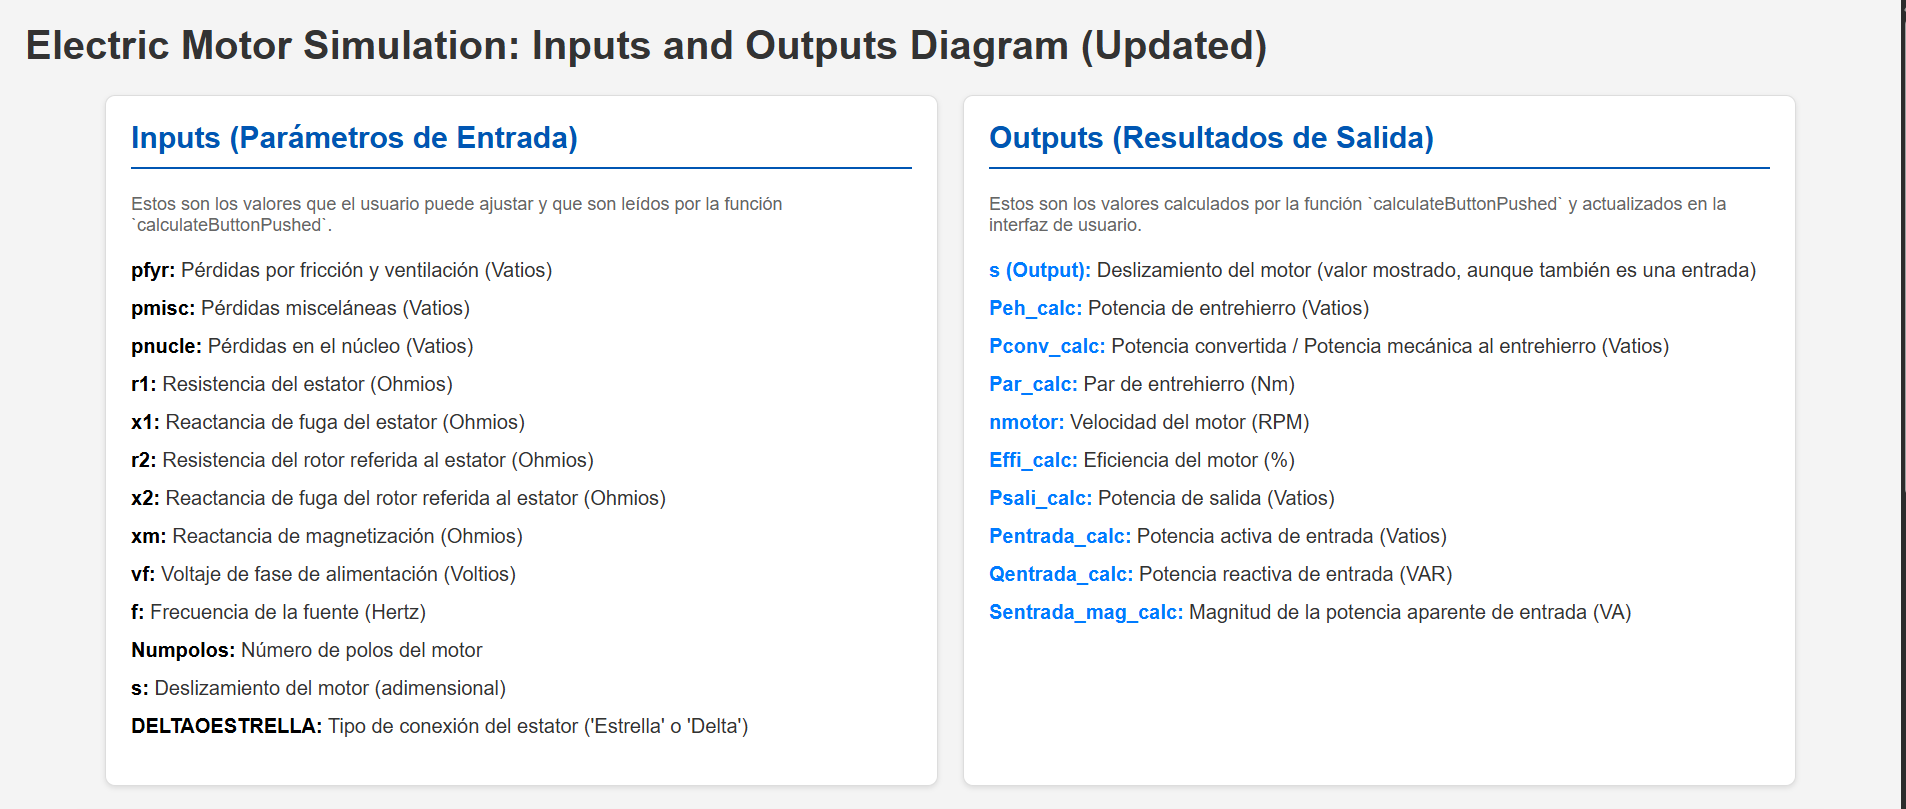
\includegraphics[width=0.48\textwidth]{imginterfaz/identificandoEntradas.png}
    \caption{Entradas y Salidas.\label{fig:identificandoEntradas}}
\end{figure}
En la figura \ref*{fig:identificandoEntradas} se menciona calculateButtonPushed, dicho botón que iniciará el funcionamiento de la interfaz.




\begin{figure}[ht!]
    \centering
    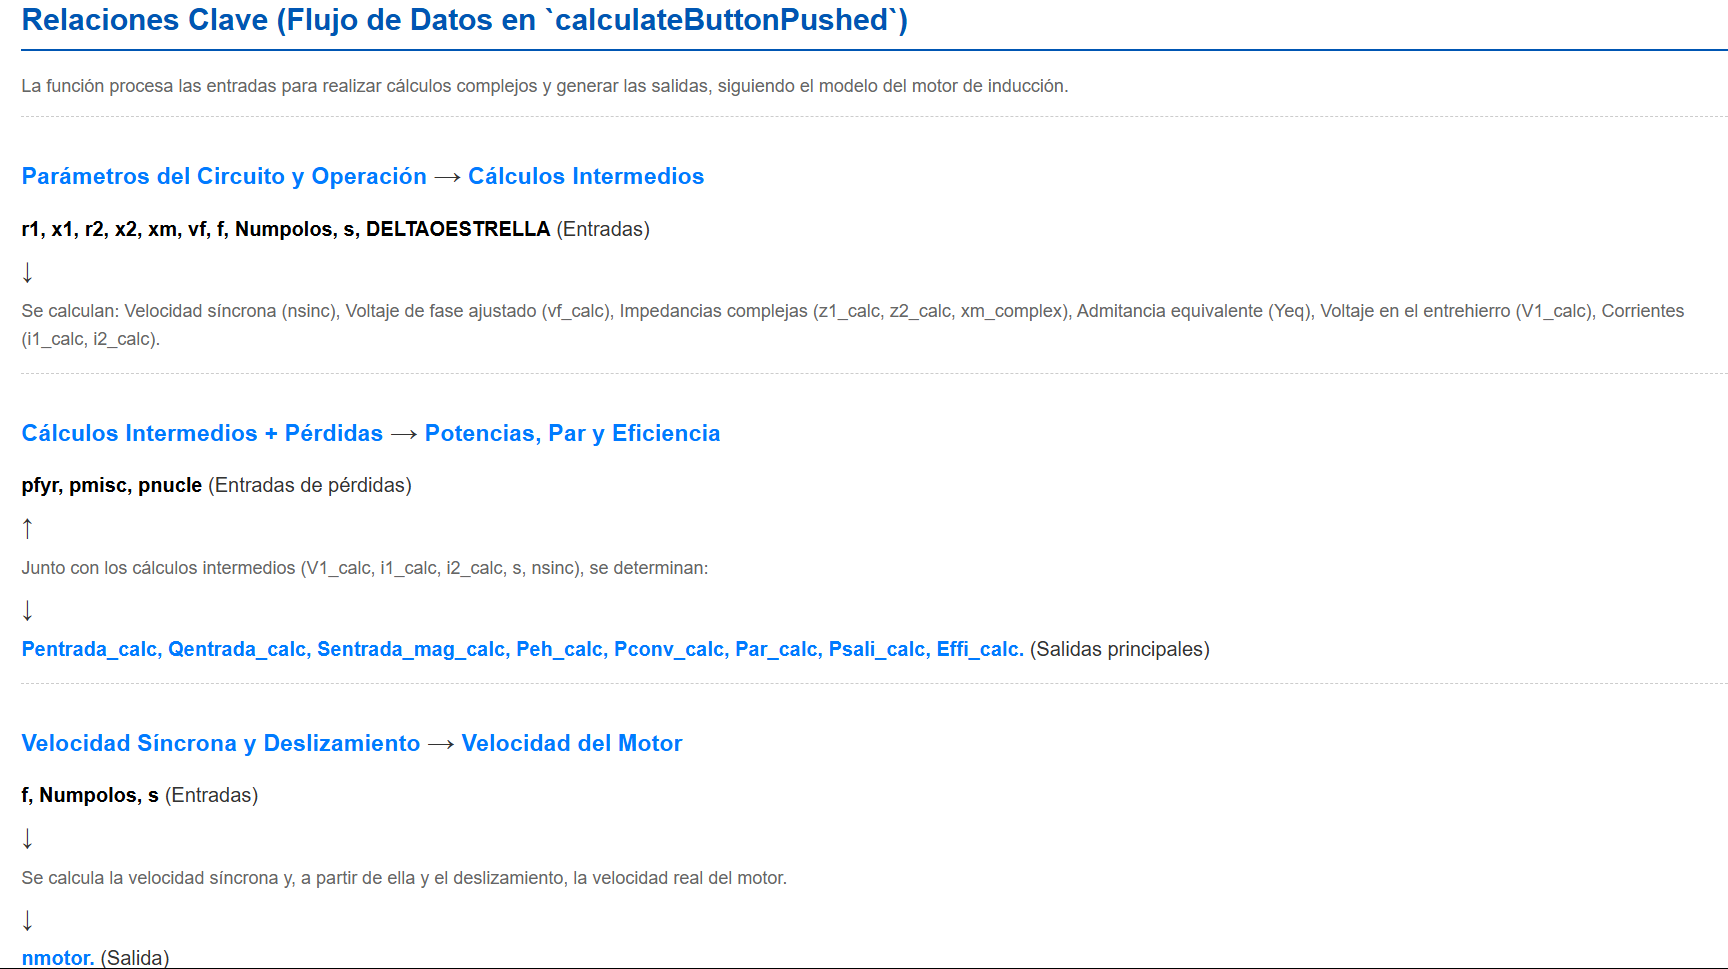
\includegraphics[width=0.48\textwidth]{imginterfaz/button.png}
    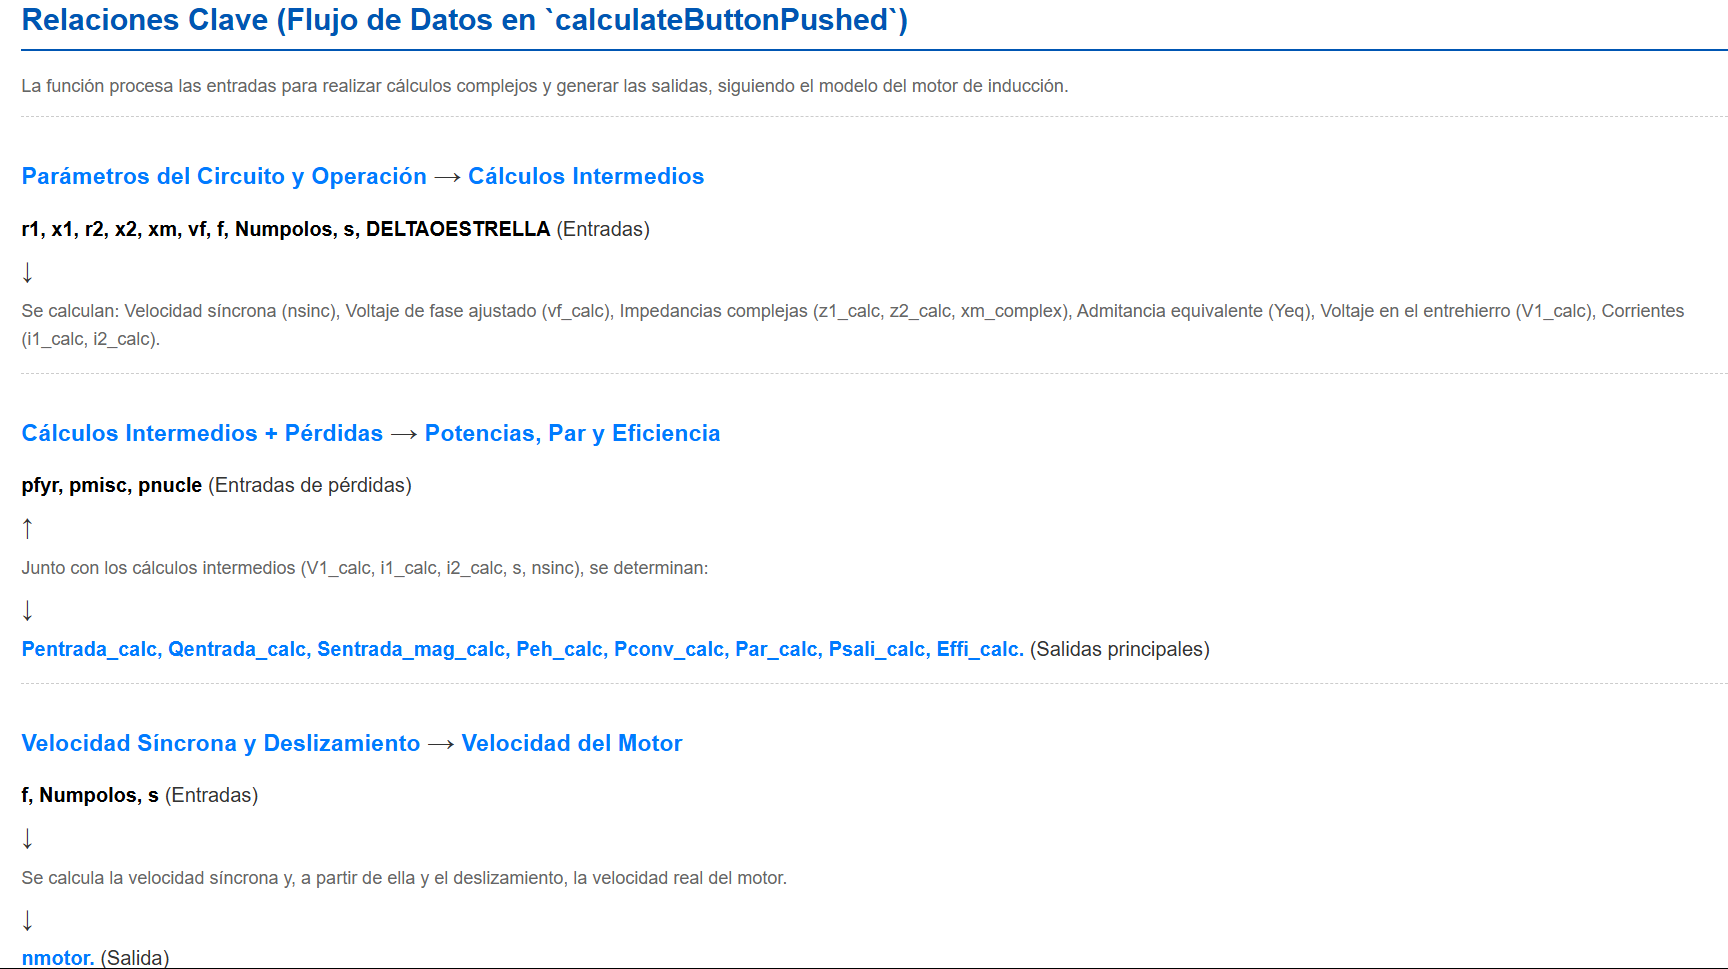
\includegraphics[width=0.48\textwidth]{imginterfaz/button.png}
    \caption{Flujo de datos de las entradas para obetener las salidas.\label{fig:button}}
\end{figure}

De la figura \ref*{fig:button} se puede observar que el flujo de datos de manera muy simplificada es el siguiente:
\begin{itemize}
    \item Se ingresan los valores de las entradas.
    \item Se presiona el botón de calcular.
    \item Se ejecuta la función que calcula los valores de salida.
    \item Se muestran los resultados en la interfaz.
    \item Se grafican los resultados.
\end{itemize}


\subsection{Aspectos relacionados con la intefaz}
En la construccion de la interfaz primero se partio del diseño de la misma, teniendo en cuenta los parametros ademas de elementos como 2 sliders y editores de texto numericos tanto para las variables de entrada como de salida.
   



Finalmente se puede observar el diseño de la interfaz con las entradas y salidas con sus respectivas unidades.
\begin{figure}[ht!]
    \centering
    \includegraphics[width=0.48\textwidth]{imginterfaz/interfaz.png}
    \caption{Interfaz de usuario.}
    \label{fig:interfaz}
\end{figure}
        \section{Diseno y aspectos relacionados con la programacion}

Se creo una función global que lee cada una de las entradas y a partir de las ecuaciones haya los parametros de la salida: 


\begin{lstlisting}[language=Matlab, caption={MATLAB Code}, basicstyle=\footnotesize\ttfamily]
function calculateButtonPushed(app, event)
    try
        % 1. Limpiar mensajes anteriores
        app.MessageBox.Text = '';
        app.MessageBox.Visible = 'off';
        % Asegurate de que los nombres de las propiedades (ej. .Value)

        % y los nombres de los componentes (ej. .pfyrEditField) sean correctos.
        pfyr = app.pfyrEditField.Value;
        pmisc = app.pmiscEditField.Value;
        pnucle = app.pnucleEditField.Value;
        r1 = app.r1EditField.Value;
        x1 = app.x1EditField.Value;
        r2 = app.r2EditField.Value;
        x2 = app.x2EditField.Value;
        xm = app.XmEditField.Value;
        vf = app.vfEditField.Value;
        f = app.fEditField.Value;
        Numpolos = app.NumpolosEditField.Value;
        s = app.sEditField.Value; % Deslizamiento (input)
        % Determinar el tipo de conexión (Estrella o Delta)
        % Asume que DELTAOESTRELLADropDown es un DropDown con 'Estrella' y 'Delta'
        if strcmp(app.DELTAOESTRELLAEditField.Value, 'Estrella')
            DELTAOESTRELLA = 0; % Estrella
        else % 'Delta'
            DELTAOESTRELLA = 1; % Delta
        end
        % 3. Validación de entradas
        % Se valida que los valores sean positivos y que Numpolos y s no sean cero.
        if any([pfyr, pmisc, pnucle, r1, x1, r2, x2, xm, vf, f, Numpolos] < 0) || Numpolos == 0
            % Si alguna entrada es negativa o Numpolos es cero.
            uialert(app.UIFigure, 'Por favor, asegúrese de que todas las entradas sean valores numéricos válidos y positivos. El número de polos no puede ser cero.', 'Error de Entrada', 'Icon', 'error');
            % Limpiar campos de salida en caso de error
            clearOutputFields(app);
            return;
        end
        % Validación específica para el deslizamiento 's'
        if s == 0
            uialert(app.UIFigure, 'Advertencia: El deslizamiento (s) es cero. Esto implica que el motor está funcionando a velocidad síncrona. Algunas ecuaciones de potencia y par pueden resultar en cero.', 'Advertencia de Deslizamiento', 'Icon', 'warning');
            % Si s es 0, r2/s sería infinito. En un motor real, s nunca es exactamente 0 con carga.
            % Sin embargo, si el usuario explícitamente pone s=0, se asume que no hay carga.
            % MATLAB puede manejar inf, pero los resultados físicos podrían no ser los esperados.
            % Para evitar NaN en los cálculos, si s es muy pequeño, podemos forzar un mínimo.
            % Pero si el usuario pone 0, se deja que MATLAB maneje el inf/nan si ocurre.
            % Aquí, se permite s=0 y se calcula, pero se advierte.
        elseif s < 0
            uialert(app.UIFigure, 'Advertencia: El deslizamiento (s) es negativo. Esto indica operación de frenado o generación. Los resultados pueden no ser típicos de operación motora.', 'Advertencia de Deslizamiento', 'Icon', 'warning');
        end
        % 4. Cálculos principales del motor
        % Velocidad síncrona (RPM)
        nsinc = 120 * f / Numpolos;
        % Velocidad del motor (RPM)
        % Si s=1, nmotor será 0, como se especifica en el requisito.
        nmotor = nsinc * (1 - s);
        % Voltaje de fase (vf_calc) según la conexión
        if DELTAOESTRELLA == 0 % Cuando es cero es estrella
            vf_calc = vf / sqrt(3);
        else % Conexión Delta
            vf_calc = vf;
        end
        % Impedancias complejas
        z1_calc = r1 + 1j * x1;
        % z2_calc: Si s es 0, r2/s será Inf, MATLAB lo maneja.
        z2_calc = (r2 / s) + 1j * x2;
        xm_complex = 1j * xm;
        % Calcular V1, I1, I2 numéricamente
        % Ecuación del nodo V1: (V1 - vf) / z1 + V1 / (j*xm) + V1 / z2 = 0
        % V1 * (1/z1 + 1/(j*xm) + 1/z2) = vf / z1
        % V1 = (vf / z1) / (1/z1 + 1/(j*xm) + 1/z2)
        % Admitancia equivalente vista desde V1
        Yeq = (1 / z1_calc) + (1 / xm_complex) + (1 / z2_calc);
        % Voltaje V1 en el entrehierro
        V1_calc = (vf_calc / z1_calc) / Yeq;
        % Corrientes
        i1_calc = (V1_calc-vf_calc)/z1_calc; % Corriente del estator
        i2_calc = V1_calc/z2_calc; % Corriente del rotor referida al estator
        % Calcular Potencia de Entrada (Pentrada) y Potencia de Entrehierro (Peh)
        % Potencia compleja de entrada (fuente de voltaje)
        % La fórmula original del usuario tiene un signo negativo: Sentrada_calc = -3 * vf_calc * conj(i1_calc);
        Sentrada_calc = -3 * vf_calc * conj(i1_calc);
        Pentrada_calc = real(Sentrada_calc);         % Potencia activa de entrada
        Qentrada_calc = imag(Sentrada_calc);         % Potencia reactiva de entrada
        Sentrada_mag_calc = abs(Sentrada_calc);      % Magnitud de la potencia aparente de entrada
        % Peh se puede calcular de dos formas: Pentrada - Pcu1 - Pnucle O 3*abs(i2)^2*r2/s
        % Usaremos la segunda forma ya que i2 y s son conocidos
        Peh_calc = 3*abs(i2_calc)^2 * r2 / s;
        % Calcular Potencia Convertida (Pconv)
        Pconv_calc = 3*abs(i2_calc)^2*r2*(1-s)/s;
        % Esto es equivalente a: Pconv_calc = Peh_calc * (1 - s);
        % Calcular Par de Entrehierro (Par)
        Par_calc = Peh_calc / (nsinc * 2 * pi / 60);
        % Calcular Potencia de Salida (Psali) y Eficiencia (Effi)
        % Psali = Pconv - Pérdidas por fricción y ventilación - Pérdidas misceláneas - Pérdidas en el núcleo
        Psali_calc = Pconv_calc - pfyr - pmisc - pnucle;
        % Eficiencia
        Effi_calc = (Psali_calc / Pentrada_calc) * 100;
        if Pentrada_calc <= 0 || isnan(Effi_calc) || isinf(Effi_calc)
            Effi_calc = 0; % Evitar división por cero o resultados no numéricos
            if Pentrada_calc <= 0
                app.MessageBox.Text = 'Advertencia: La potencia activa de entrada es cero o negativa. La eficiencia no se puede calcular o no es aplicable.';
                app.MessageBox.FontColor = [0.85 0.33 0.1]; % Naranja
                app.MessageBox.Visible = 'on';
            end
        end
        % 5. Actualizar campos de salida de la UI
        app.sOutputEditField.Value = s; % Mostrar el deslizamiento de entrada
        app.pehEditField.Value = Peh_calc;
        app.pconvEditField.Value = Pconv_calc;
        app.parEditField.Value = Par_calc;
        app.nmotorEditField.Value = nmotor;
        app.effiEditField.Value = Effi_calc;
        app.psalEditField.Value = Psali_calc;
        app.PentradaEditField.Value = Pentrada_calc;
        app.QentradaEditField.Value = Qentrada_calc;
        app.SentradaEditField.Value = Sentrada_mag_calc;
        % Mostrar mensaje de éxito
        app.MessageBox.Text = 'Cálculos completados exitosamente.';
        app.MessageBox.FontColor = [0 0.5 0]; % Verde
        app.MessageBox.Visible = 'on';
        % --- NUEVOS CÁLCULOS PARA GRAFICAR LA CURVA COMPLETA ---
        sgrafica = -1:0.001:1; % Rango de deslizamiento, por ejemplo
        nmotorgraf = nsinc .* (1 - sgrafica);
        % ... (el resto de tus cálculos vectoriales para z2_graf, V1_calcgraf, i2_calc_graf, Peh_graf, Par_calcgraf) ...
        z2_graf = (r2 ./ sgrafica) + 1j * x2;
        Yeqgraf = (1 ./ z1_calc) + (1 ./ xm_complex) + (1 ./ z2_graf);
        V1_calcgraf = (vf_calc ./ z1_calc)./Yeqgraf;
        i2_calc_graf = V1_calcgraf ./ z2_graf;
        Peh_graf = 3 * abs(i2_calc_graf).^2 * r2 ./ sgrafica;
        Par_calcgraf = Peh_graf ./ (nsinc .* 2 * pi / 60);
        % --- CÓDIGO DE GRAFICACIÓN DIRECTO ---
        cla(app.updateMotorPlots); % Limpia la gráfica anterior
        plot(app.updateMotorPlots, nmotorgraf, Par_calcgraf, '-', 'LineWidth', 0.8);
        xlabel(app.updateMotorPlots, 'Velocidad del Motor (RPM)');
        ylabel(app.updateMotorPlots, 'Par del Motor (Nm)');
        title(app.updateMotorPlots, 'Curva Característica: Par vs. Velocidad');
        grid(app.updateMotorPlots, 'on');
        hold(app.updateMotorPlots, 'on');
        % --- Segunda gráfica
        plot(app.updateMotorPlots, nmotor, Par_calc, 'r-o', 'DisplayName', 'Potencia de Salida', 'LineWidth', 1.5); % Línea roja con guiones y 'x'
        % 3. Restaurar el comportamiento predeterminado de los ejes
        hold(app.updateMotorPlots, 'off');
        cla(app.desli); % Limpia la gráfica anterior
        plot(app.desli, sgrafica, Par_calcgraf, '-', 'LineWidth', 0.8);
        xlabel(app.desli, 'Deslizamiento');
        ylabel(app.desli, 'Par del Motor (Nm)');
        title(app.desli, 'Curva Característica: Par vs. Deslizamiento');
        grid(app.desli, 'on');
        hold(app.desli, 'on');
        plot(app.desli, s, Par_calc, 'r o', 'DisplayName', 'Deslizamiento', 'LineWidth', 1.5); % Línea roja con guiones y 'x'
        hold(app.desli, 'off');
        % --- Aquí es donde agregas la llamada a la función de graficación ---
        % Los parámetros s_values, Psali_results, s_single, Par_at_s_single,
        % Psali_at_s_single, nmotor_at_s_single se pasan para que la función
        % updateMotorPlots tenga todos los datos que espera, incluso si para
        % esta gráfica específica solo usamos nmotor y Par_calc.
        % Si updateMotorPlots espera vectores, puedes convertir los valores
        % escalares a vectores de un solo elemento:
    catch ME
        % 6. Manejo de errores
        % Mostrar mensaje de error al usuario
        uialert(app.UIFigure, ['Error en el cálculo: ' ME.message], 'Error', 'Icon', 'error');
        app.MessageBox.Text = ['Error: ' ME.message];
        app.MessageBox.FontColor = [1 0 0]; % Rojo
        app.MessageBox.Visible = 'on';
        % Limpiar campos de salida en caso de error
        clearOutputFields(app);
    end
end
% --- Función auxiliar para limpiar campos de salida ---
function clearOutputFields(app)
    app.sOutputEditField.Value = 0;
    app.pehEditField.Value = 0;
    app.pconvEditField.Value = 0;
    app.parEditField.Value = 0;
    app.nmotorEditField.Value = 0;
    app.effiEditField.Value = 0;
    app.psalEditField.Value = 0;
    app.PentradaEditField.Value = 0;
    app.QentradaEditField.Value = 0;
    app.SentradaEditField.Value = 0;
end
% --- Función de inicio de la aplicación (StartupFcn) ---
% (Opcional) Puedes usar esta función para establecer valores predeterminados
% al iniciar la aplicación.
function StartupFcn(app)
    % Establecer valores predeterminados para los campos de entrada
    app.pfyrEditField.Value = 1500;
    app.pmiscEditField.Value = 1500;
    app.pnucleEditField.Value = 450;
    app.r1EditField.Value = 0.012;
    app.x1EditField.Value = 0.41;
    app.r2EditField.Value = 0.25;
    app.x2EditField.Value = 0.32;
    app.XmEditField.Value = 4.6;
    app.vfEditField.Value = 440;
    app.fEditField.Value = 60;
    app.NumpolosEditField.Value = 4;
    app.sEditField.Value = (1800-1740)/1800; % Deslizamiento inicial
    % Establecer la opción predeterminada para el DropDown
    app.DELTAOESTRELLAEditField.Items = {'Estrella', 'Delta'};
    app.DELTAOESTRELLAEditField.Value = 'Delta';
    % Inicializar campos de salida como vacíos o NaN
    clearOutputFields(app);
    % Ocultar el cuadro de mensajes al inicio
    app.MessageBox.Visible = 'off';
end
\end{lstlisting}






        \section{Pruebas con la interfaz}
la interfaz fue probada con el siguiente ejemplo:
\begin{figure}[ht!]
    \centering
    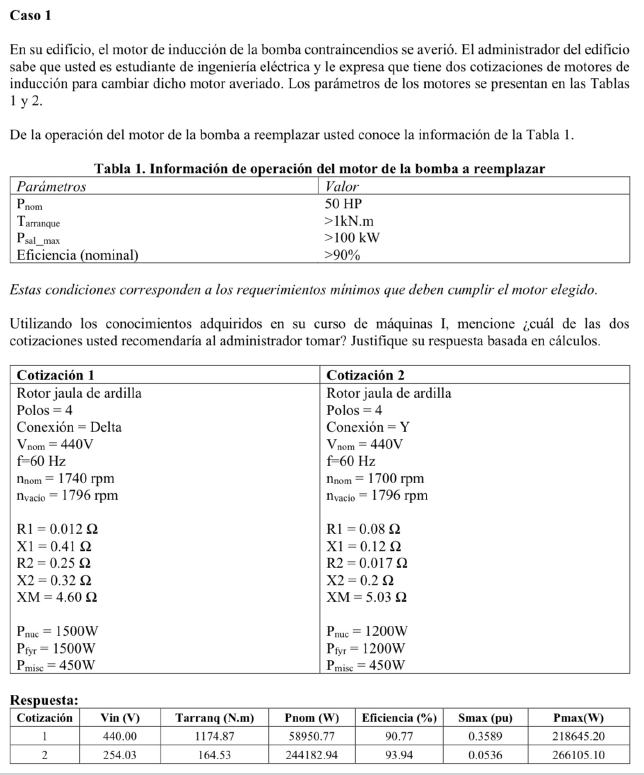
\includegraphics[width=0.48\textwidth]{imginterfaz/Ejemplo.png}
    \caption{Ejemplo para poner a prueba la interfaz.}
    \label{fig:Ejemplo}
\end{figure}


En donde los resultados de la interfaz fueron los siguientes:
\begin{figure}[ht!]
    \centering
    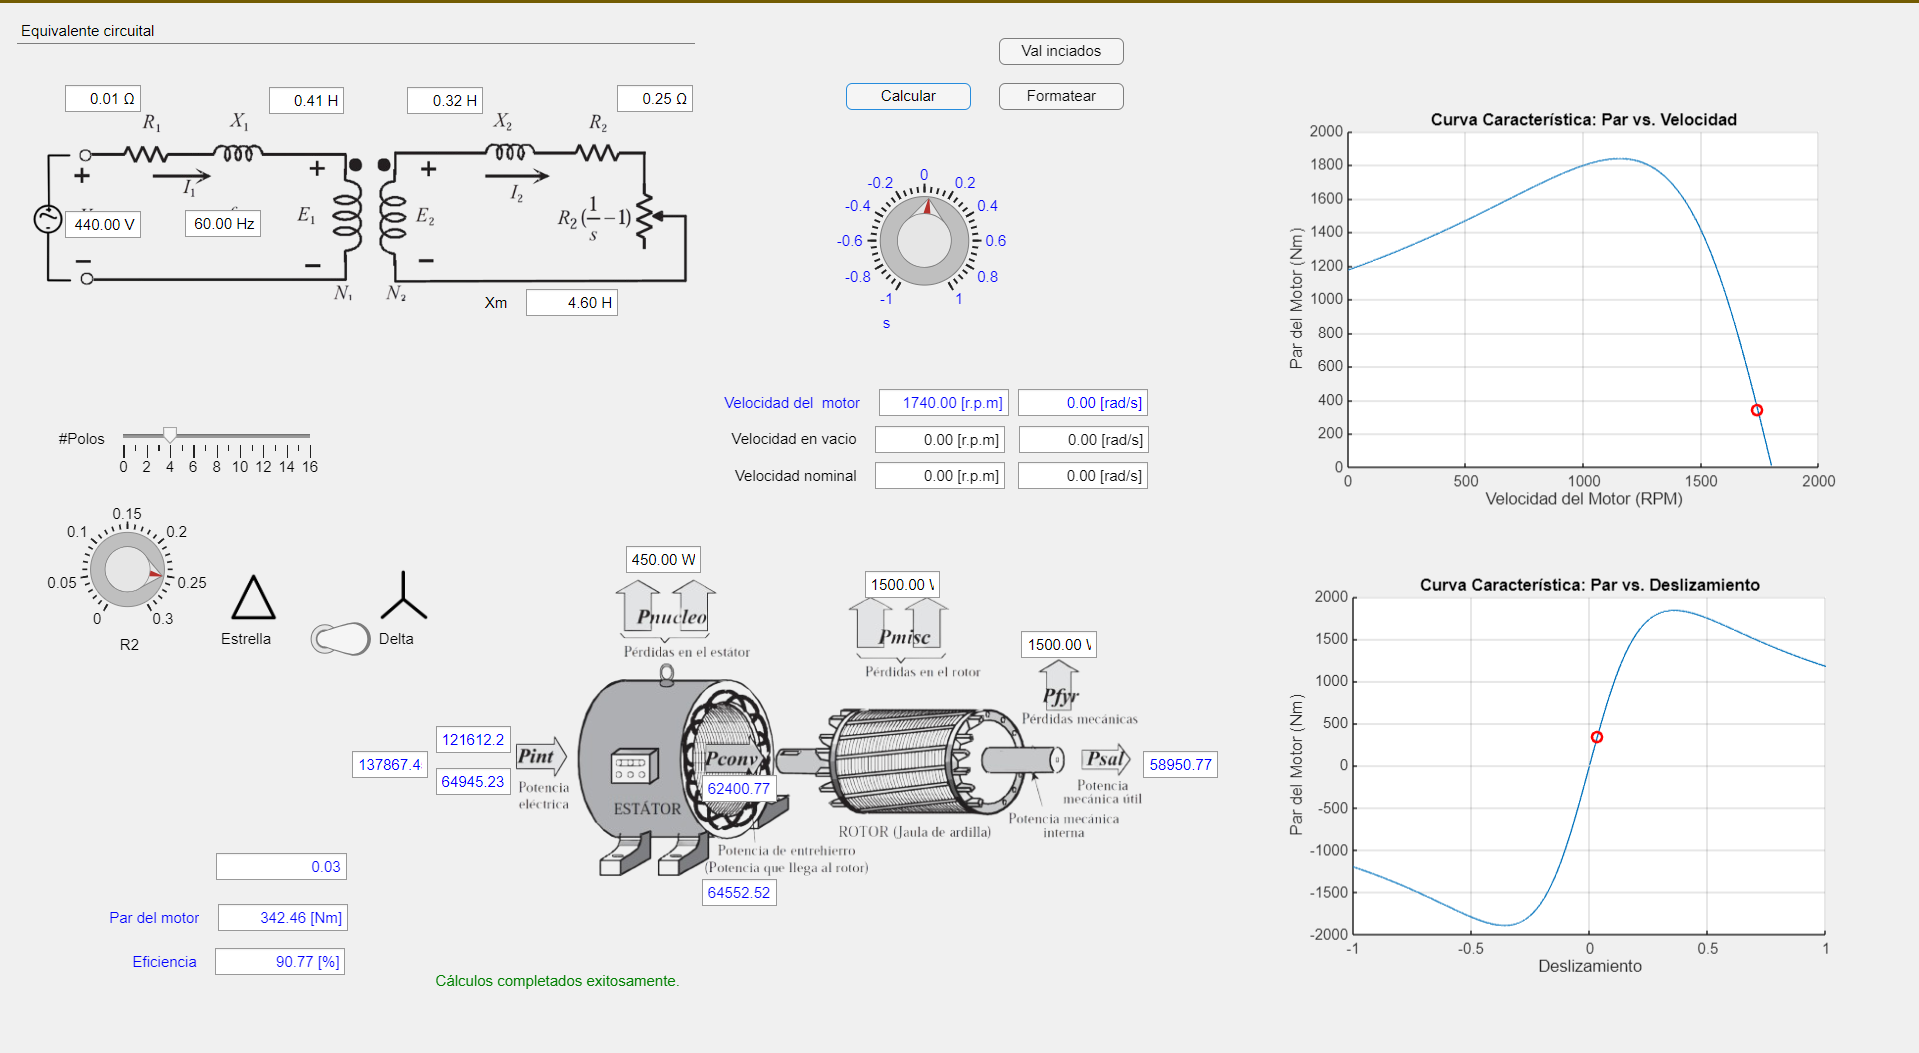
\includegraphics[width=0.48\textwidth]{imginterfaz/resultados (2).png}
    \caption{Resultados de la interfaz al ejemplo.}
    \label{fig:resultado}
\end{figure}

         % Add the bibliography file in the preamble (correct usage)
        %\section*{Nomenclature}
        %    \addcontentsline{toc}{section}{Nomenclature}
        %    \begin{IEEEdescription}[\IEEEsetlabelwidth{$V_1,V_2,$}]
        %    \item[\smash{\begin{IEEEeqnarraybox*}[][t]{l}
        %    V_1,V_2,\\
        %    \hphantom{V_1,{}}V_3
        %    \end{IEEEeqnarraybox*}}] Three-phase PWM output line voltages.\\
        %    \mbox{}
        %    \item[$\theta$] Rotor angle (in ``electrical degrees'').
        %    \item[$\omega$] Rotor (electrical) speed, corresponding to the time
        %    derivative of $\theta$.
        %    \end{IEEEdescription}

        %    \begin{IEEEitemize}
        %        \item First item
        %        \item Second item
        %    \end{IEEEitemize}

            
        %    \begin{IEEEenumerate}
        %        \item First item
        %        \item Second item
        %    \end{IEEEenumerate}
        %    
        %    \begin{IEEEdescription}
        %        \item First item
        %        \item Second item
        %    \end{IEEEdescription}


        %   \begin{IEEEproof}
        %        The statement is true.
        %   \end{IEEEproof}


        
            \section{Conclusiones}
            La interfaz desarrollada mostro un resultado conciso y claro. Con relación a los resultados fueron los esperados, aunque como adicional se podria hacer que en las graficas se mostrara la velocidad cuando el motor opera como generador para la grafica Par del motor velocidad del motor no lo logre sin embargo para la grafica deslizamiento del motor y par del motor si.


            \begin{thebibliography}{1}
                
                \bibitem{Fitzgerald2020}
                A. E. Fitzgerald, C. Kingsley, y A. Kusko, \emph{Electric Machinery}, 7ª ed. Nueva York, EE. UU.: McGraw-Hill Education, 2020.
                \label{Fitzgerald2020}


                \bibitem{Fraile2008}
                J. Fraile Mora, \emph{Máquinas Eléctricas}, 6ª ed. Madrid, España: McGraw-Hill, 2008.
                \label{Fraile2008}

            \end{thebibliography}

        \end{document}  